\chapter{Equipment Health Assessment using Artificial Neural Networks}
%\chapter{Classification of Healthy and Faulty States using Neural Networks}

\chapterintrobox{Ce chapitre démontre l'utilisation d'un réseau de neurones artificiels pour estimer l'état de santé d'un ensemble de turbosoufflantes à partir de l'ensemble de données C-MAPSS de la NASA et prédire la durée de vie utile restante. Il présente également différentes mesures permettant d'évaluer les performances du réseau.}

\section{Introduction à la base de données C-MAPSS}

C-MAPSS est un outil de simulation de grands turboréacteurs commerciaux réalistes. Le logiciel est codé dans l'environnement MATLAB\textsuperscript{\textregistered} et Simulink\textsuperscript{\textregistered}.

\begin{wrapfigure}{r}{0.5\textwidth}
    \centering
    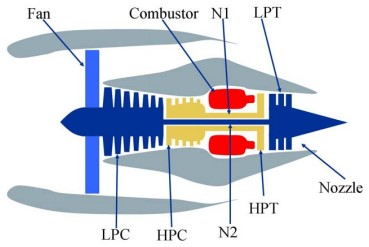
\includegraphics[width=.48\textwidth]{figures/c-mapss-engine-diagram.jpg}
    \caption{Schéma simplifié d'un turboréacteur simulé dans C-MAPSS \cite{Saxena2008}}
    \label{figure:c-mapss-engine-diagram}    
\end{wrapfigure}

Le logiciel C-MAPSS est composé de nombreux paramètres d'entrée éditables qui contrôlent la simulation. Ces entrées sont spécifiées par l'utilisateur et contrôlent de nombreux aspects de la simulation tels que le profil opérationnel, les contrôleurs en boucle fermée, les conditions environnementales, etc. \cite{Saxena2008}. 

La figure \ref{figure:c-mapss-engine-diagram} est un diagramme simplifié du turboréacteur simulé montrant ses principaux éléments, comme la section de compresseur basse pression (LPC), la section de compresseur haute pression (HPC), la soufflante et la chambre de combustion. L'ensemble de données publié par le Centre de recherche Ames de la NASA contient les données résultant de la simulation de nombreux turboréacteurs, depuis le début du fonctionnement jusqu'à la panne. L'ensemble de données a été initialement publié pour la compétition de Pronostics et gestion de la santé 2008. Le tableau \ref{table:c-mapss-sensors} montre différentes variables, la sortie de la simulation et leurs unités, qui ont été fournies pour les participants à la compétition :

\begin{table}[ht]
    \centering
    \begin{tabu}{lll}
		\tabucline[1.5pt]{-} 
        \textbf{Symbol} & \textbf{Description} & \textbf{Units}\\
        \hline
        \textbf{T2} & Total temperature at fan inlet & R \\
        \textbf{T24} & Total temperature at LPC outlet & R \\
        \textbf{T30} & Total temperature at HPC outlet & R  \\
        \textbf{T50} &Total temperature at LPT & R\\
        \textbf{P2} & Pressure at fan inlet& psia\\
        \textbf{P15}& Total pressure in bypass-duct& psia\\
        \textbf{P30}& Total pressure at HPC outlet& psia\\
        \textbf{Nf}& Physical fan speed& rpm\\
        \textbf{Nc} & Physical core speed &rpm\\
        \textbf{epr}& Engine pressure ratio (P50/P2)& --\\
        \textbf{Ps30}& Static pressure at HPC outlet& psia\\
        \textbf{phi}& Ratio of fuel flow to Ps30& pps/psi\\
        \textbf{NRf}& Corrected fan speed &rpm\\
        \textbf{NRc}& Corrected core speed& rpm\\
        \textbf{BPR}& Bypass Ratio& --\\
        \textbf{farB}& Burner fuel-air ratio &--\\
        \textbf{htBleed}& Bleed Enthalpy &-- \\
        \textbf{Nf\_dmd} &Demanded fan speed& rpm\\
        \textbf{PCNfR\_dmd}& Demanded corrected fan speed &rpm\\
        \textbf{W31} & HPT coolant bleed & lbm/s \\
        \textbf{W32} & LPT coolant bleed & lbm/ \\
		\tabucline[1.5pt]{-} 
    \end{tabu}
    \caption{Sortie de simulation C-MAPSS pour mesurer la réponse du système}
    \label{table:c-mapss-sensors}
\end{table}

La base de données C-MAPSS contient 4 ensembles : FD001, FD002, FD003 et FD004. Chaque ensemble a des conditions de travail et des modes de défaillance différents. Le tableau \ref{table:c-mapss-statistics} contient les statistiques des différents ensembles :

\begin{table}[ht]
    \centering
    \begin{tabu}{ccccc}
        
		\tabucline[1.5pt]{2-5} 
                    & units number  & max length    & average length    & min length    \\
       \hline
            FD001   & 100           & 362           & 206.31            & 128           \\
            FD002   & 260           & 378           & 206.77            & 128           \\
            FD003   & 100           & 525           & 247.2             & 145           \\
            FD004   & 249           & 543           & 245.95            & 128           \\
		\tabucline[1.5pt]{-} 
    \end{tabu}
    \caption{Statistiques sur le nombre d'unités et la longueur des cycles dans la base de données C-MAPSS.}
    \label{table:c-mapss-statistics}
\end{table}

\section{Visualisation de la dégradation des turboréacteurs}
La visualisation des résultats de la simulation peut donner une idée de la façon dont ces variables changent pendant la durée de vie du turboréacteur. La figure \ref{fig:sensors-plot} montre quatre capteurs différents de l'un des moteurs (les valeurs sont normalisées) :

\begin{figure}[h]
    \centering
    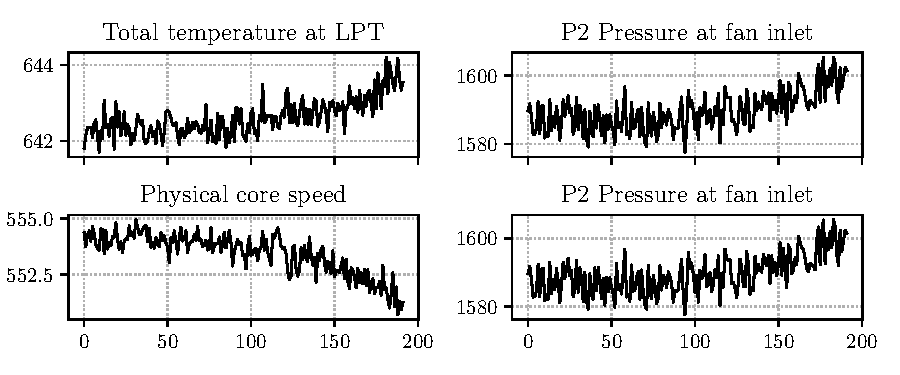
\includegraphics[width=\linewidth]{figures/sensors_plot.pdf}
    \caption{Développement de 6 capteurs de sortie d'un des turboréacteurs (normalisé)}
    \label{fig:sensors-plot}
\end{figure}
\begin{figure}[H]
    \centering
    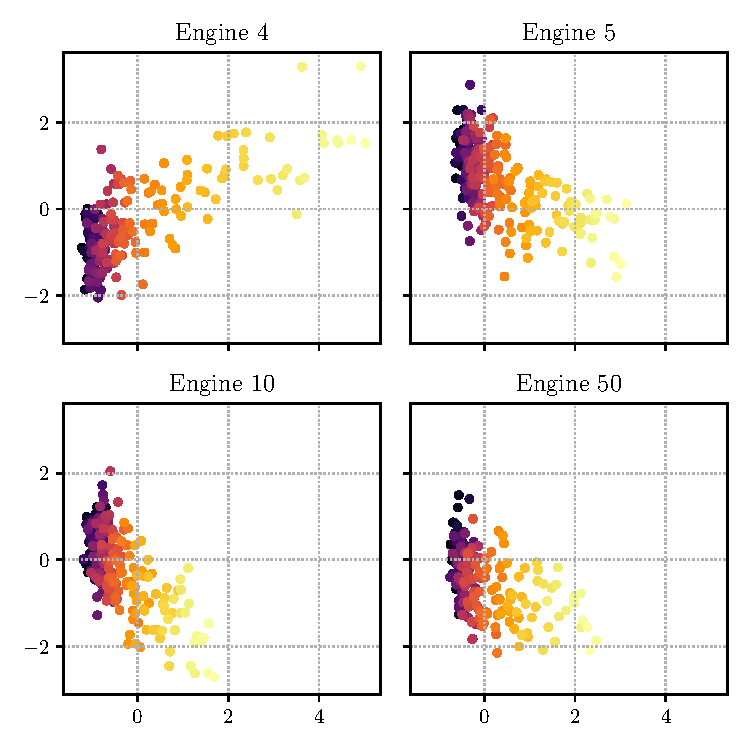
\includegraphics[width=.9\linewidth]{figures/pca-degradation.pdf}
    \caption{Dégradation de la santé de l'équipement (des couleurs plus claires indiquent l'avancement de la dégradation de la santé) de quatre turboréacteurs à partir de la base de données C-MAPSS}
    \label{fig:pca-degradation}
\end{figure}

Il est évident que la sortie des capteurs suit un tendance spécifique (croissant ou décroissant) du début de l'opération jusqu'à la panne, ce qui est très utile et peut augmenter la fiabilité du modèle prédictif.

Alternativement, toutes les valeurs des capteurs peuvent être combinées et visualisées ensemble en utilisant l'analyse en composantes principales (section \ref{section:dimensionality-reduction}) pour révéler la tendance générale des données. Si les données de surveillance de l'état de santé de l'équipement sont directement indicatives de l'état de santé de l'équipement, la visualisation des composantes principales peut montrer des modèles de dégradation visuelle apparents.

Les valeurs des capteurs de 4 turboréacteurs différents sont combinées à l'aide de l'ACP et les deux premiers composants principaux sont représentés sur la figure \ref{fig:pca-dégradation}. 

Il existe un schéma absolument apparent de dégradation de l'état de santé dans les différentes unités, de la gauche (où les couleurs plus foncées indiquent un état de fonctionnement normal) à la droite (où les couleurs plus claires indiquent le développement de défauts).

\section{classification de l'état de santé des turboréacteurs}
Avant de procéder à une tâche compliquée telle que l'estimation \acrshort{rul}, une tâche plus simple comme la classification sanitaire des turboréacteurs peut montrer la complexité du problème. Cette section décrit l'utilisation des réseaux de neurones pour classer les états des moteurs comme étant sains ou défectueux. Les 25 premiers et derniers cycles de chaque unité sont considérés comme sains et défectueux respectivement.

Un réseau de neurones qui utilise les 24 entrées (tous les paramètres opérationnels et les capteurs) avec deux couches cachées est utilisé pour effectuer cette classification. Le tableau \ref{table:c-mapss-classifier-architecture} résume l'architecture du réseau :

\begin{table}[ht]
    \centering
    \begin{tabu}{lll}
		\tabucline[1.5pt]{-}
		\textbf{Layer (type)}   & \textbf{Output shape} &   \textbf{Param \#} \\
		\tabucline[1pt]{-}
		Dense1 (Dense) 			&   (None, 8)   &   200\\
		Dense2 (Dense) 	        &   (None, 4)   &   36       \\
		Dense3 (Dense)			&   (None, 1)   &   5   \\
		\tabucline[1pt]{-}
		Total params: 241       &                   &           \\
		Trainable params: 241   &                   &           \\
		Non-trainable params: 0     &                   &           \\
	\tabucline[1.5pt]{-}
    \end{tabu}
    \caption{Architecture du classificateur de l'état des unités}
    \label{table:c-mapss-classifier-architecture}
\end{table}

Le modèle est entraîné pour 200 époques avec batch size de 32 échantillons, le classificateur atteint une précision de \textbf{93,46\%} sur les données de test. La figure \ref{fig:cmapss-classifier-training} montre le processus d'entraînement du réseau. Dans le diagramme du haut, l'axe des y correspond aux pertes d'entraînement et de validation (crossentropie binaire). L'axe des y dans le diagramme du bas correspond aux précisions d'entraînement et de validation du réseau, l'axe des x partagé entre les deux diagrammes indique les époques de formation. Bien que la précision de validation varie beaucoup, la précision d'entraînement continue de s'améliorer à chaque époque.

\begin{figure}[H]
    \centering
    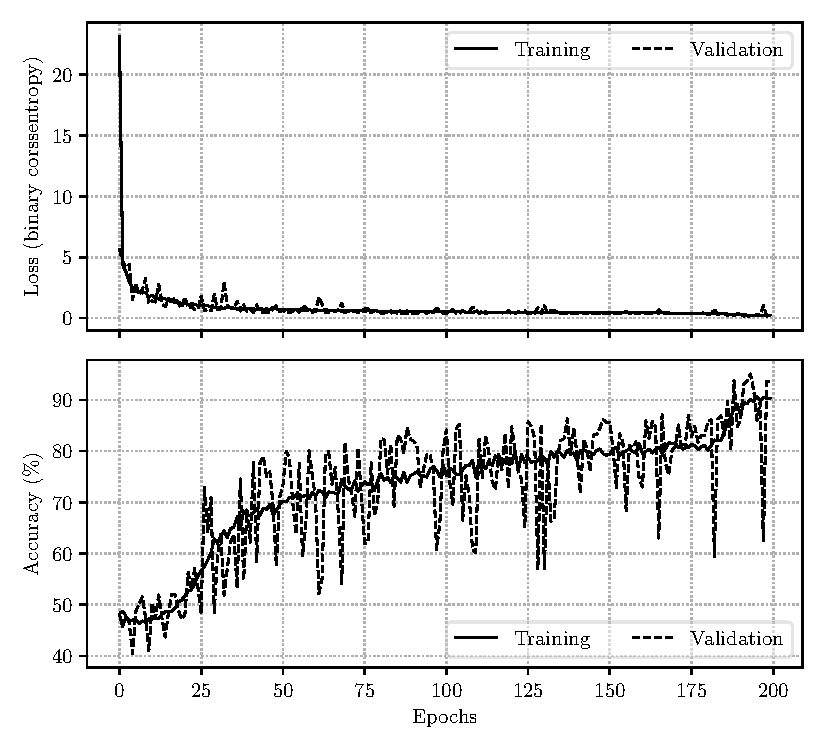
\includegraphics{figures/cmapss_classification_training.pdf}
    \caption{Processus d'entraînement du classificateur de l'état des unités}
    \label{fig:cmapss-classifier-training}
\end{figure}

La figure \ref{fig:cmapss-classifier-roc} montre la courbe \acrlong{roc} (\acrshort{roc}) du classificateur avec un haut \acrlong{auc} (\acrshort{auc}). D'autres mesures de classification sont présentées dans le tableau \ref{table:cmapss-classifier-metrics}.

\begin{figure}[H]
    \centering
    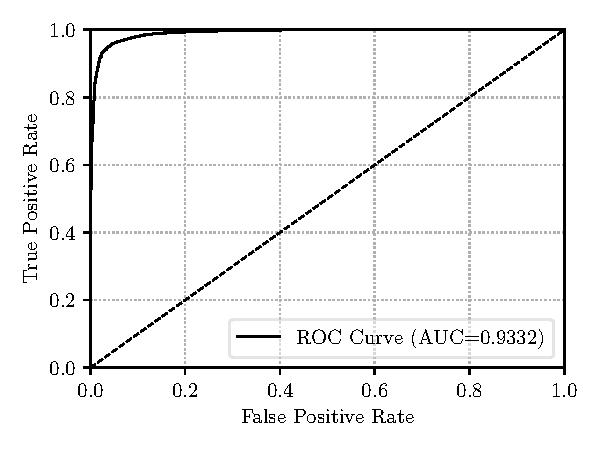
\includegraphics{figures/cmapss_classification_roc.pdf}
    \caption{Courbe \acrshort{roc} du classificateur sur les données de test}
    \label{fig:cmapss-classifier-roc}
\end{figure}

\begin{table}[H]
    \centering
    \begin{tabu}{cccccc}
        
    \tabucline[1.5pt]{-}
    \textbf{Metric} &  \textbf{Accuracy} &  \textbf{Precision} &  \textbf{Recall} &  \textbf{F-1} &  \textbf{ROC AUC}  \\
    \hline
    \textbf{Score} & 93.43\% & 0.90 & 0.98 & 0.94 & 0.9332 \\
	\tabucline[1.5pt]{-}
    \end{tabu}
    \caption{Métriques du classificateur sur les données de test}
    \label{table:cmapss-classifier-metrics}
\end{table}

\section{Prédiction de \acrshort{rul}}
\subsection{Modèlisation de \acrshort{rul}}

Afin d'entraîner un réseau de neurones pour l'estimation de  \acrlong{rul} (\acrshort{rul}) d'une nouvelle donnée non vue provenant de base de données C-MAPSS, un \acrshort{rul} approprié correspondant aux données d'entraînement doit être construit.

L'expression \acrshort{rul} a été définie dans la section \ref{section:rul}, à partir de cette définition, plusieurs approches pour construire un \acrshort{rul} approprié peuvent être développées pour les unités dans les données d'entraînement (où le nombre total de cycles avant la défaillance est connu). L'approche la plus simple consiste à utiliser un \acrshort{rul} toujours décroissant, ce qui implique que l'état de l'équipement est toujours décroissant et va vers la défaillance.

Le problème de cette approche est que le processus de dégradation n'est pas linéaire et que dans la vie réelle, les machines ne commencent pas à se dégrader dès qu'elles commencent à fonctionner. Une deuxième approche consiste à utiliser une fonction par morceaux où l'état de l'équipement est d'abord constant puis, à un point spécifique, il commence à se dégrader de manière linéaire.

Cette approche est bien meilleure que la première, mais elle n'est pas très représentative du comportement réel du processus de dégradation. Dans le contexte de ce mémoire, \acrshort{rul} est abordé comme une fonction polynomiale non linéaire où la dégradation est lente au début puis s'accélère vers la fin de la vie. La figure \ref{fig:rul-models} montre les différents choix de modélisation de \acrshort{rul} :

\begin{figure}[H]
    \centering
    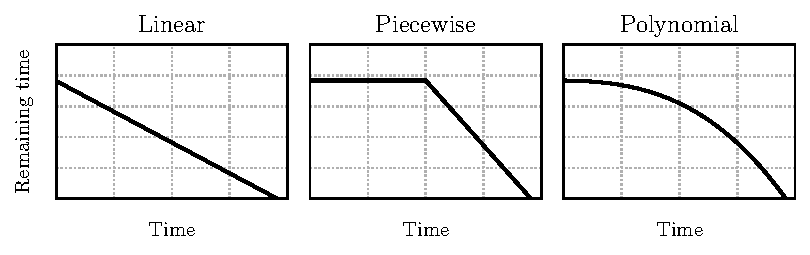
\includegraphics{figures/rul_models.pdf}
    \caption{Différents modèles de \acrshort{rul}}
    \label{fig:rul-models}
\end{figure}

Il convient de noter qu'aucune de ces approches ne peut être considérée comme représentative du processus de dégradation réel, mais le choix de la représentation la plus intuitive de \acrshort{rul} peut aider l'algorithme d'apprentissage à connaître les tendances de dégradation implicites dans les données.

\subsection{Prédiction de \acrshort{rul} par un réseau de neurones}

La dernière section portait sur la classification de l'état de santé des unités comme étant sain ou défectueux. Cette section présente plutôt un réseau de neurones pour l'estimation de la \acrshort{rul}. Dans cette section, une architecture de réseau de neurones avec 3 couches cachées est utilisée. Comme il s'agit d'un problème de régression, l'erreur quadratique moyenne est utilisée comme fonction de perte, l'erreur absolue moyenne est utilisée comme mesure pour le modèle. Le tableau \ref{table:cmapss-regression-architecture} présente les détails de l'architecture :

\begin{table}[h]
    \centering
    \begin{tabu}{lll}
		\tabucline[1.5pt]{-}
		\textbf{Layer (type)}   & \textbf{Output shape} &   \textbf{Param \#} \\
		\tabucline[1pt]{-}
		Dense1 (Dense) 			&   (None, 32)  &       800     \\
		Dense2 (Dense)          &   (None, 16)  &       528     \\
		Dense3 (Dense)          &   (None, 8)   &       136     \\
		Dense4 (Dense)          &   (None, 1)   &       9       \\

		\tabucline[1pt]{-}
		Total params: 1,473       &                   &           \\
		Trainable params: 1,473   &                   &           \\
		Non-trainable params: 0   &                   &           \\
	\tabucline[1.5pt]{-}
    \end{tabu}
    \caption{Architecture d'un réseau de neurones pour la prédiction de \acrshort{rul}}
    \label{table:cmapss-regression-architecture}
\end{table}

Le réseau a été entraîné pour 300 époques, avec batch size de 128 échantillons. La figure \ref{fig:cmapss-regression-formation} montre le processus de'entraînement du réseau. Les figures montrent l'évolution des pertes d'entraînement et de validation (erreur quadratique moyenne) et des métriques (erreur absolue moyenne) respectivement en fonction des époques.

\begin{figure}[H]
    \centering
    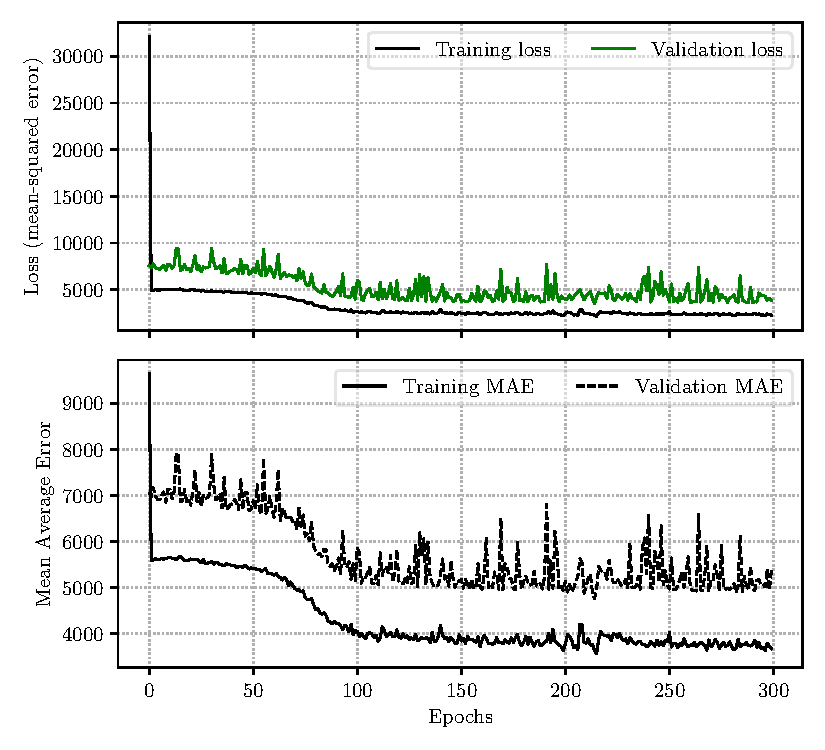
\includegraphics{figures/cmapss_regression_training.pdf}
    \caption{Processus d'entraînement du réseau utilitsé pour prédire \acrshort{rul}}
    \label{fig:cmapss-regression-training}
\end{figure}

Après l'entraînement, le modèle est évalué sur deux unités de la série de tests. La figure \ref{fig:cmapss-regression-prédiction} montre le \acrshort{rul} réel (ligne discontinue), la prédiction du modèle à chaque cycle et un ajustement polyomial de 3ème degré des prédictions du modèle.

\begin{figure}[H]
    \centering
    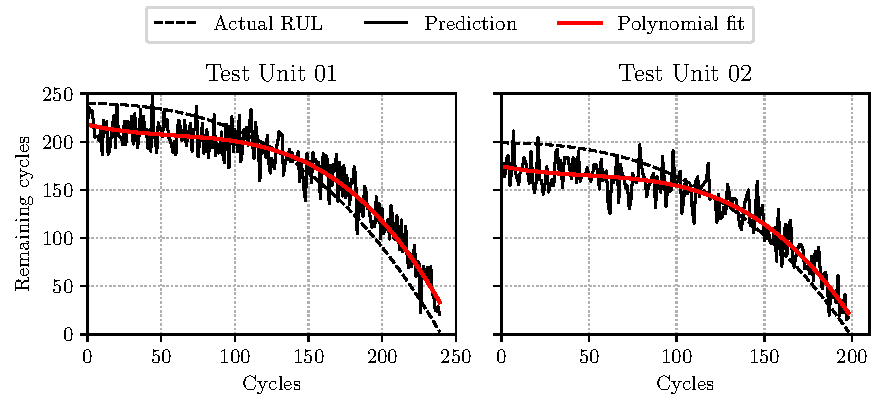
\includegraphics{figures/cmapss_regression_predictions.pdf}
    \caption{Résultats de prédiction de \acrshort{rul} par un réseau de neurones}
    \label{fig:cmapss-regression-prediction}
\end{figure}

Although the model's prediction are close the the actual \acrshort{rul}, but they are noisy and there is so much fluctuation. The noise can be reduced by smoothing the output for example using moving average or fitting the points to a polynomial. But the reason of the noise in the first place is that fully-connected architecture doesn't take into consideration the previous predictions (i.e. acyclic architecture). Since \acrshort{rul} at each instant of time depends on the \acrshort{rul} from the previous one, taking previous steps into consideration while making new predictions can effectively reduce the noise and also improve prediction accuracy. To achieve that, a cyclic neural archtiecture like recurrent neural networks should be used.

\subsection{Amélioration de la prédiction \acrshort{rul} en utilisant les réseaux LSTM}

Les réseaux de neurones entièrement connectés constituent un outil puissant pour la modélisation d'un large éventail de problèmes, mais l'utilisation de cette architecture pour la prédiction de séries chronologiques, comme la prédiction \acrshort{rul}, peut donner un résultat très bruyant car le réseau est acyclique et chaque instant dans le temps est évalué séparément et ne tient pas compte des prédictions précédentes. \acrlong{lstm} (Section \ref{section:lstm}) est un outil puissant pour modéliser de tels problèmes et pour faire des prédictions plus fiables et moins bruyantes. Dans cette section, l'architecture de réseau de neurones entièrement connectée de la section précédente est remplacée par un réseau \acrshort{lstm} pour prédire \acrshort{rul} des turboréacteurs de la base de données C-MAPSS.

L'architecture utilisée ici est décrite dans le tableau \ref{table:cmapss-lstm-architecture}:

\begin{table}[h]
    \centering
    \begin{tabu}{lll}
		\tabucline[1.5pt]{-}
		\textbf{Layer (type)}   & \textbf{Output shape} &   \textbf{Param \#} \\
		\tabucline[1pt]{-}
		LSTM1 (LSTM) 			&   (None, 100, 100)    &       50000   \\
		LSTM2 (LSTM)           &   (None, 100, 100)    &       80400   \\
		LSTM3 (LSTM)           &   (None, 75)          &       52800   \\
        Dense1 (Dense)         &   (None, 120)         &       9120    \\
        Dense2 (Dense)         &   (None, 110)         &       13310   \\
        Dense3 (Dense)         &   (None, 100)         &       11100   \\
		\tabucline[1pt]{-}
		Total params: 216,730       &                   &               \\
		Trainable params: 216,730   &                   &               \\
		Non-trainable params: 0     &                   &               \\
	\tabucline[1.5pt]{-}
    \end{tabu}
    \caption{Architecture de réseau \acrshort{lstm} pour la prédiction de \acrshort{rul}}
    \label{table:cmapss-lstm-architecture}
\end{table}

Il est évident que l'architecture \acrshort{lstm} a beaucoup plus de paramètres (216,730 paramètres) que l'architecture entièrement connectée (1,473). Cela est dû à la conception plus complexe des cellules \acrshort{lstm} et à leur possession de différentes portes. Il en résulte un temps d'entraînement beaucoup plus long.

Les couches \acrshort{lstm} prennent un tenseur tridimensionnel de la forme \textit{(samples, sequence length, features)} comme entrée. La longueur de la séquence a été fixée à 100 dans cette architecture, c'est pourquoi chaque échantillon d'entraînement doit avoir une forme de \textit{(sequence length, features)}. Toutes les unités ont le même nombre de caractéristiques mais des longueurs différentes, puisque chaque échantillon doit avoir une longueur de séquence de 100, les échantillons avec des cycles inférieurs à 100 sont complétés par -10 où les couches \acrshort{lstm} sont définies pour ignorer tout les instants de temps avec cette valeur.

Le réseau a été entraîné pour 50 époques avec batch size de 16 échantillons et un fractionnement de validation de 0,2 en utilisant l'algorithme d'optimization Adam. Le processus d'entraînement est visualisé sur la figure \ref{fig:cmapss-lstm-training} :

\begin{figure}[H]
    \centering
    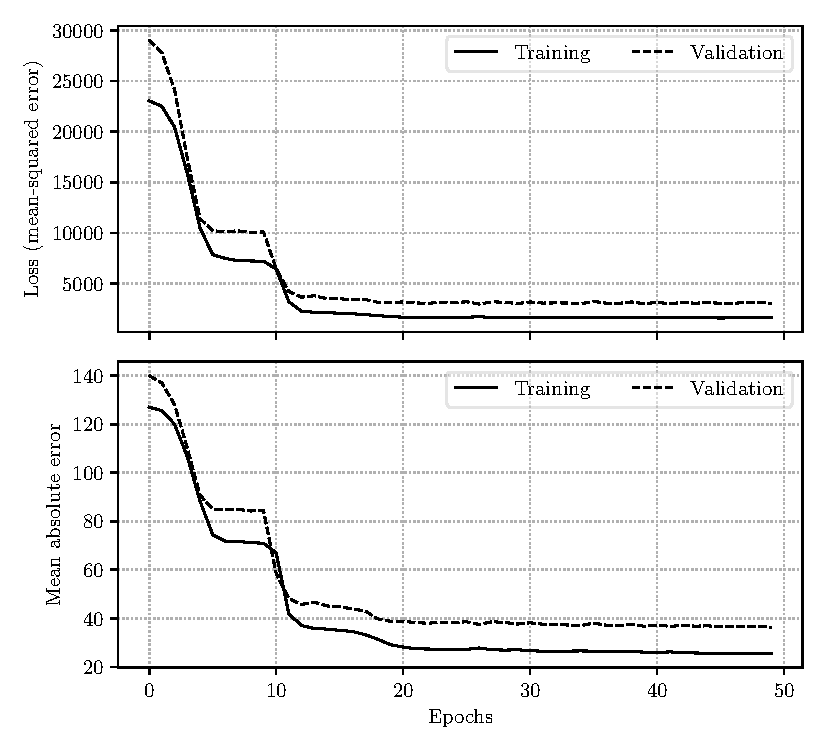
\includegraphics{figures/cmapss_lstm_training.pdf}
    \caption{Processus d'entraînement du réseau \acrshort{lstm}}
    \label{fig:cmapss-lstm-training}
\end{figure}

Le tableau \ref{tableau:cmapss-lstm-results} montre la perte et la métrique (c'est-à-dire l'erreur absolue moyenne) sur les donnée d'entraînement, validation et de test :

\begin{table}[H]
	\centering
	\begin{tabu}{lcc}
		\tabucline[1.5pt]{2-3} 
						&	\textbf{Loss}	&	\textbf{Mean Absolute Error}	\\
	   \tabucline[1pt]{-}
		Train set 		&	1600.60			    &	25.43				\\
		Validation set 	&	3039.68 			&	36.37					\\
		Test set		&	1379.67 			&	23.27					\\
   \tabucline[1.5pt]{-}
   \end{tabu}
   \caption{Résultats d'entraînement du réseau\acrshort{lstm}}
   \label{table:cmapss-lstm-results}
\end{table}

Quatre unités différentes ont été réservées comme unités de test. Après l'entraînement, le réseau est utilisé pour prédire \acrshort{rul} sur les unités de test. La figure \ref{fig:cmapss-lstm-prediction} montre les résultats de la prédiction et la \acrshort{rul} réelle de deux unités différentes :

\begin{figure}[h]
    \centering
    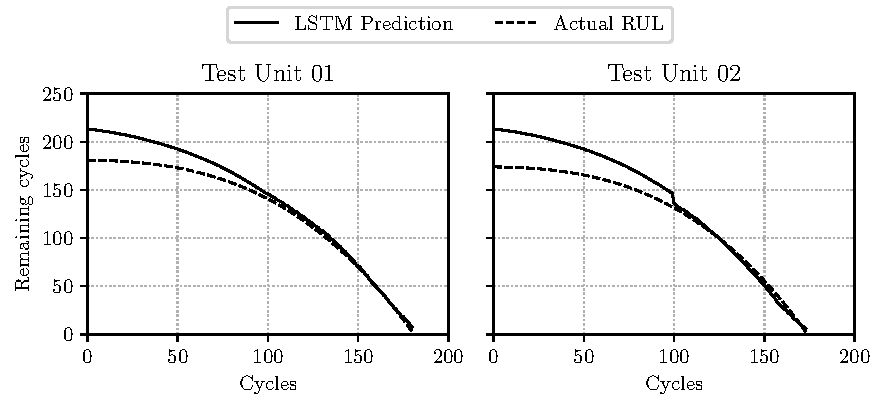
\includegraphics{figures/cmapss_lstm_regression_predictions.pdf}
    \caption{Résultats de prédiction du réseau \acrshort{lstm}}
    \label{fig:cmapss-lstm-prediction}
\end{figure}

Il est évident que les prédictions du réseau \acrshort{lstm} sont bien meilleures et presque exemptes de bruit par rapport à celles faites par le réseau entièrement connecté, comme le montre la figure \ref{fig:cmapss-regression-prediction}. La prédiction \acrshort{rul} est presque identique à la prédiction réelle \acrshort{rul} vers la fin de vie du turboréacteur.

\section{Conclusion}
Les réseaux de neurones entièrement connectés sont un outil puissant pour quantifier l'état de santé de systèmes complexes à l'aide de données de surveillance des conditions. L'ensemble de données C-MAPSS est un exemple de système comportant de nombreuses parties en interaction qui fournissent une variété de données de surveillance de l'état de santé (par exemple, la température, la pression, le régime, ...) où la dégradation n'est pas directement liée à une composante mais est indiquée par la somme des tendances de toutes les données de surveillance. Les réseaux de neurones sont capables de saisir de telles tendances et de prédire \acrshort{rul} du système avant une défaillance. Les réseaux entièrement connectés ont d'abord été utilisés pour cette tâche, mais une architecture cyclique comme \acrshort{lstm} peut produire de meilleurs résultats avec une précision accrue et beaucoup moins de bruit.

\begin{comment}
\chapter{Equipment Health Assessment using Artificial Neural Networks}
%\chapter{Classification of Healthy and Faulty States using Neural Networks}

\chapterintrobox{This chapter demonstrates the use of an artificial neural network to estimate the health state of a set of turbofan engines from NASA C-MAPSS dataset and predict the remaining useful life. Also different metrics to assess the performance of the network will be introduced.}

\section{Introduction to NASA C-MAPSS dataset}

C-MAPSS is a tool for simulating a realistic large commercial turbofan engine. The software is coded in the MATLAB\textsuperscript{\textregistered} and Simulink\textsuperscript{\textregistered} environment.

\begin{wrapfigure}{r}{0.5\textwidth}
    \centering
    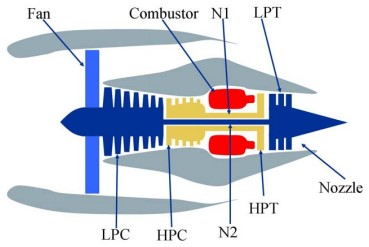
\includegraphics[width=.48\textwidth]{figures/c-mapss-engine-diagram.jpg}
    \caption{Simplified diagram of engine simulated in C-MAPSS \cite{Saxena2008}}
    \label{figure:c-mapss-engine-diagram}    
\end{wrapfigure}

C-MAPSS software consists of many editable input parameters that controls the simulation, these inputs are specified by the user and control many aspects of the simulation such as operational profile, closed-loop controllers, environmental conditions, etc. \cite{Saxena2008}. 

Figure \ref{figure:c-mapss-engine-diagram} is a simplified diagram of the simulated engine showing its main elements, like low pressure compressor section (LPC), high pressure compressor section (HPC), fan and combustor. The dataset released by NASA Ames Research Center contains resulting data from simulating many turbofan engines, from beginning of operation until failure. The dataset was originally released for Prognostics and Health Management 2008 Data Competition, Table \ref{table:c-mapss-sensors} shows different variables, the output of the simulation and their units, that were provided for the participants in the competition:

\begin{table}[ht]
    \centering
    \begin{tabu}{lll}
		\tabucline[1.5pt]{-} 
        \textbf{Symbol} & \textbf{Description} & \textbf{Units}\\
        \hline
        \textbf{T2} & Total temperature at fan inlet & R \\
        \textbf{T24} & Total temperature at LPC outlet & R \\
        \textbf{T30} & Total temperature at HPC outlet & R  \\
        \textbf{T50} &Total temperature at LPT & R\\
        \textbf{P2} & Pressure at fan inlet& psia\\
        \textbf{P15}& Total pressure in bypass-duct& psia\\
        \textbf{P30}& Total pressure at HPC outlet& psia\\
        \textbf{Nf}& Physical fan speed& rpm\\
        \textbf{Nc} & Physical core speed &rpm\\
        \textbf{epr}& Engine pressure ratio (P50/P2)& --\\
        \textbf{Ps30}& Static pressure at HPC outlet& psia\\
        \textbf{phi}& Ratio of fuel flow to Ps30& pps/psi\\
        \textbf{NRf}& Corrected fan speed &rpm\\
        \textbf{NRc}& Corrected core speed& rpm\\
        \textbf{BPR}& Bypass Ratio& --\\
        \textbf{farB}& Burner fuel-air ratio &--\\
        \textbf{htBleed}& Bleed Enthalpy &-- \\
        \textbf{Nf\_dmd} &Demanded fan speed& rpm\\
        \textbf{PCNfR\_dmd}& Demanded corrected fan speed &rpm\\
        \textbf{W31} & HPT coolant bleed & lbm/s \\
        \textbf{W32} & LPT coolant bleed & lbm/ \\
		\tabucline[1.5pt]{-} 
    \end{tabu}
    \caption{C-MAPSS outputs to measure system response.}
    \label{table:c-mapss-sensors}
\end{table}

C-MAPSS data contains 4 datasets: FD001, FD002, FD003 and FD004. Each dataset has different working conditions and fault modes. Table \ref{table:c-mapss-statistics} contains statistics of the different datasets:

\begin{table}[ht]
    \centering
    \begin{tabu}{ccccc}
        
		\tabucline[1.5pt]{2-5} 
                    & units number  & max length    & average length    & min length    \\
       \hline
            FD001   & 100           & 362           & 206.31            & 128           \\
            FD002   & 260           & 378           & 206.77            & 128           \\
            FD003   & 100           & 525           & 247.2             & 145           \\
            FD004   & 249           & 543           & 245.95            & 128           \\
		\tabucline[1.5pt]{-} 
    \end{tabu}
    \caption{Units number and cycles length statistics in C-MAPSS data}
    \label{table:c-mapss-statistics}
\end{table}

\section{Visualization of equipment degredation}
Visualizing the simulation output can give a sense of how these variables change during the life of the engine, Figure \ref{fig:sensors-plot} shows four different sensors from one of the engines (values are normalized):

\begin{figure}[h]
    \centering
    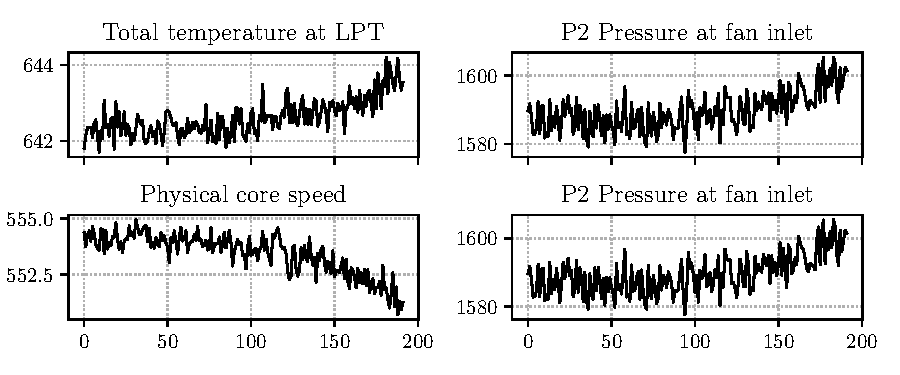
\includegraphics[width=\linewidth]{figures/sensors_plot.pdf}
    \caption{Development of 6 sensors outputs from one of the engines (normalized)}
    \label{fig:sensors-plot}
\end{figure}
\begin{figure}[H]
    \centering
    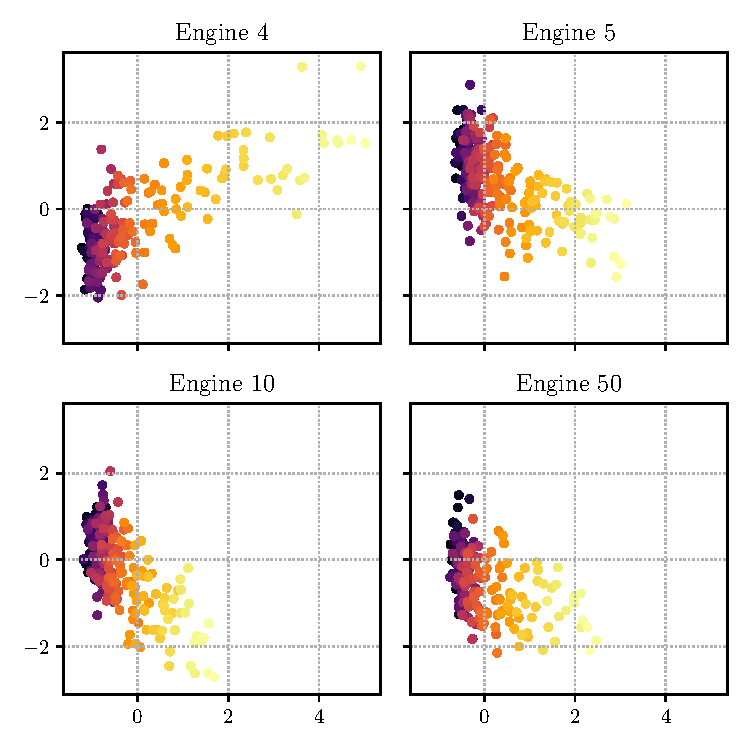
\includegraphics[width=.9\linewidth]{figures/pca-degradation.pdf}
    \caption{Equipment health degredation (lighter colors indicate advancing of health degradation) of four turbofan engines from C-MAPSS dataset}
    \label{fig:pca-degradation}
\end{figure}

It is apparent that sensors output follow a specific pattern (increasing or decreasing) from beginning of operation until breakdown, this is very useful and can increase the robustness of the predictive model.

Alternatively, all sensors values can be combined and visualized altogether using Principal Component Analysis (section \ref{section:dimensionality-reduction}) to reveal the general trend in the datat, if condition monitoring data is directly indicative of the equipment health state, visualization of principal components can show apparent visual degradation patterns.

Sensors values from 4 different engines are combined using PCA and the two first principal components are represented on Figure \ref{fig:pca-degradation}. 

There is absolutely an apparent pattern for health state degradation across the different engines from left (where darker colors indicate normal working state) to the right (where the lighter colors indicate fault development).

\section{Engines health classification}
Before proceeding with a complicated task such as \acrshort{rul} estimation, a simpler task like engines health classification can show the complexity of the problem. This section describes using neural networks to classify engines states as healty or faulty. The first and last 25 cycles from each unit are considered to be healthy and faulty respectively.

A neural network that uses all 24 inputs (all operational settings and sensors) with two hidden layers is used to carry out this classification. Table \ref{table:c-mapss-classifier-architecture} summarizes the network architecture:

\begin{table}[ht]
    \centering
    \begin{tabu}{lll}
		\tabucline[1.5pt]{-}
		\textbf{Layer (type)}   & \textbf{Output shape} &   \textbf{Param \#} \\
		\tabucline[1pt]{-}
		Dense1 (Dense) 			&   (None, 8)   &   200\\
		Dense2 (Dense) 	        &   (None, 4)   &   36       \\
		Dense3 (Dense)			&   (None, 1)   &   5   \\
		\tabucline[1pt]{-}
		Total params: 241       &                   &           \\
		Trainable params: 241   &                   &           \\
		Non-trainable params: 0     &                   &           \\
	\tabucline[1.5pt]{-}
    \end{tabu}
    \caption{C-MAPSS classifier architecture}
    \label{table:c-mapss-classifier-architecture}
\end{table}

The model is trained for 200 epochs with batch size of 32 samples, the classifier achieves \textbf{93.46\% accuracy} on the test set. Figure \ref{fig:cmapss-classifier-training} shows the training process of the network. In the upper plot, the y-axis corresponds to the train and validation losses (binary crossentropy). The y-axis in the lower plot corresponds to the network train and validation accuracies, the x-axis shared between the two plots indicates the training epochs. Although the validation accuracy varies a lot, the training accuracy keeps improving with each epoch.

\begin{figure}[H]
    \centering
    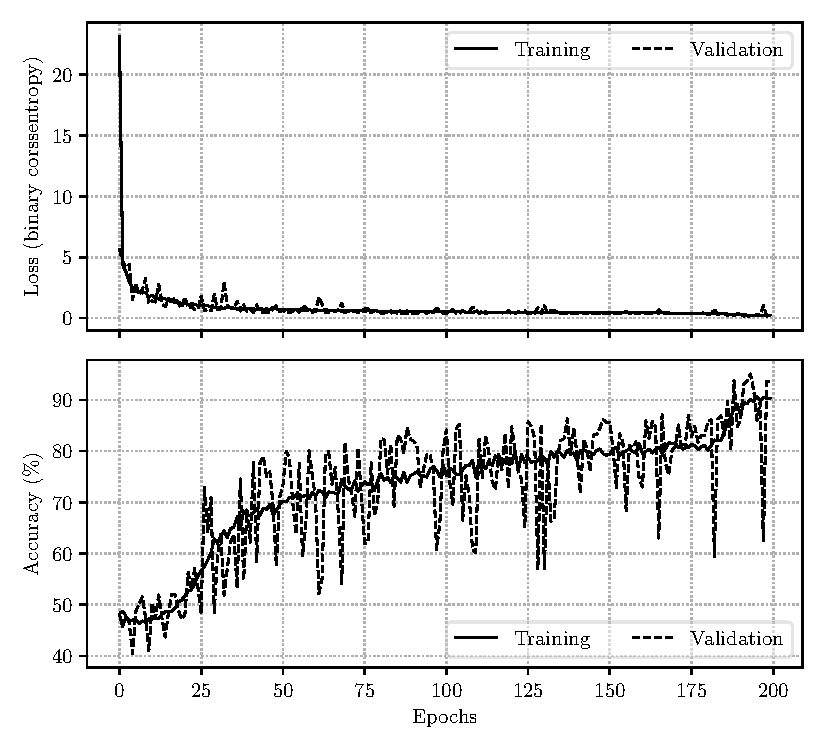
\includegraphics{figures/cmapss_classification_training.pdf}
    \caption{Training process of C-MAPSS classifier}
    \label{fig:cmapss-classifier-training}
\end{figure}

Figure \ref{fig:cmapss-classifier-roc} shows \acrlong{roc} (\acrshort{roc}) Curve of the classifier with a high \acrlong{auc} (\acrshort{auc}). Other classification metrics are shown in Table \ref{table:cmapss-classifier-metrics}.

\begin{figure}[H]
    \centering
    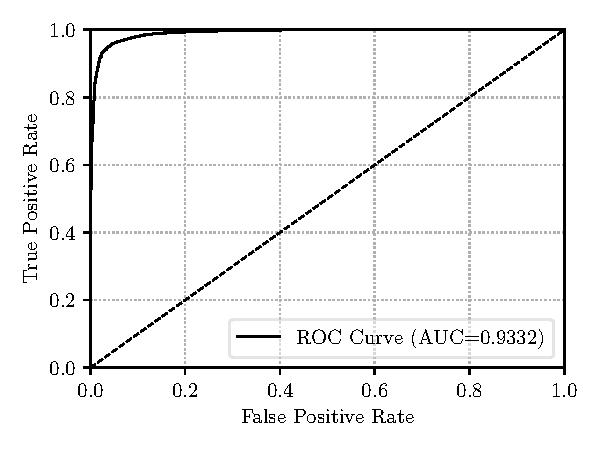
\includegraphics{figures/cmapss_classification_roc.pdf}
    \caption{C-MAPSS classifier ROC curve on test set}
    \label{fig:cmapss-classifier-roc}
\end{figure}

\begin{table}[H]
    \centering
    \begin{tabu}{cccccc}
        
    \tabucline[1.5pt]{-}
    \textbf{Metric} &  \textbf{Accuracy} &  \textbf{Precision} &  \textbf{Recall} &  \textbf{F-1} &  \textbf{ROC AUC}  \\
    \hline
    \textbf{Score} & 93.43\% & 0.90 & 0.98 & 0.94 & 0.9332 \\
	\tabucline[1.5pt]{-}
    \end{tabu}
    \caption{C-MAPSS classifier metrics on test set}
    \label{table:cmapss-classifier-metrics}
\end{table}

\section{Remaining Useful Life prediction}
\subsection{Remaining Useful Life modeling}
In order to train a neural network to estimate the \acrlong{rul} (\acrshort{rul}) of a new unseen data from C-MAPSS dataset, an appropriate \acrshort{rul} that corresponds to the training data must be constructed. \acrshort{rul} was defined in Section \ref{section:rul}, from this definition several approaches to construct an appropriate \acrshort{rul} can be developed for units in the train data (where the total number of cycles before failure is known). The simplest approach is to use an always-decreasing \acrshort{rul}, this implies that the equipment state is always decreasing and moving towards failure. The problem with this approach is that degradation process isn't linear and in real life, machines don't start to degrade as soon as they are start working. A second approach is to use a piecewise function where the equipment state is constant at first then at a specific point it starts to degrade linearly. This approach is much better than the first one but it is not very representative of the real world behaviour of degradation process. In the context of this thesis, \acrshort{rul} is approached as a nonlinear polynomial function where the degradation is slow at first then accelerates towards the end of life. Figure \ref{fig:rul-models} shows the different choices for modeling \acrshort{rul}:

\begin{figure}[H]
    \centering
    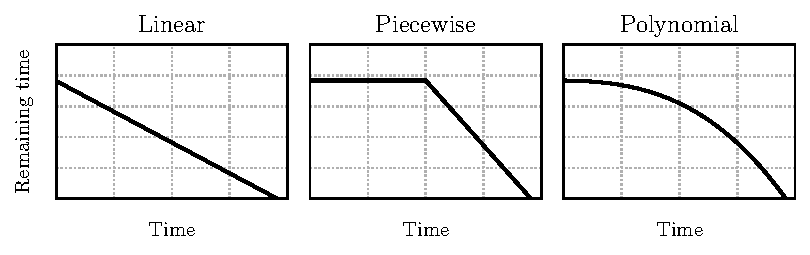
\includegraphics{figures/rul_models.pdf}
    \caption{Different \acrshort{rul} modeling choices}
    \label{fig:rul-models}
\end{figure}

It must be noted that not any of these approaches can be claimed to be representative of the real world degradation process, but choosing the most intuitive representation of \acrshort{rul} can help the learning algorithm learn the implicit degradation trends in the data.

\subsection{\acrshort{rul} prediction using feed-forward network}
The last section dealt with classifying units health state as healthy or faulty. This section instead presents a neural network for estimating the \acrshort{rul}. In this section, a neural network architecture with 3 hidden layers is used. Since this is a regression problem, mean squared error is used as the loss function, mean absolute error is used as a metric for the model. Table \ref{table:cmapss-regression-architecture} presents the architecture details:

\begin{table}[h]
    \centering
    \begin{tabu}{lll}
		\tabucline[1.5pt]{-}
		\textbf{Layer (type)}   & \textbf{Output shape} &   \textbf{Param \#} \\
		\tabucline[1pt]{-}
		Dense1 (Dense) 			&   (None, 32)  &       800     \\
		Dense2 (Dense)          &   (None, 16)  &       528     \\
		Dense3 (Dense)          &   (None, 8)   &       136     \\
		Dense4 (Dense)          &   (None, 1)   &       9       \\

		\tabucline[1pt]{-}
		Total params: 1,473       &                   &           \\
		Trainable params: 1,473   &                   &           \\
		Non-trainable params: 0   &                   &           \\
	\tabucline[1.5pt]{-}
    \end{tabu}
    \caption{Fully-connected network architecture for \acrshort{rul} prediction}
    \label{table:cmapss-regression-architecture}
\end{table}

The network was trained for 300 epochs, batch size of 128 samples. Figure \ref{fig:cmapss-regression-training} shows the training process of the network. The figures show the development of training and validation losses (mean squared error) and metrics (mean absolute error) respectively as a function of training epochs.

\begin{figure}[H]
    \centering
    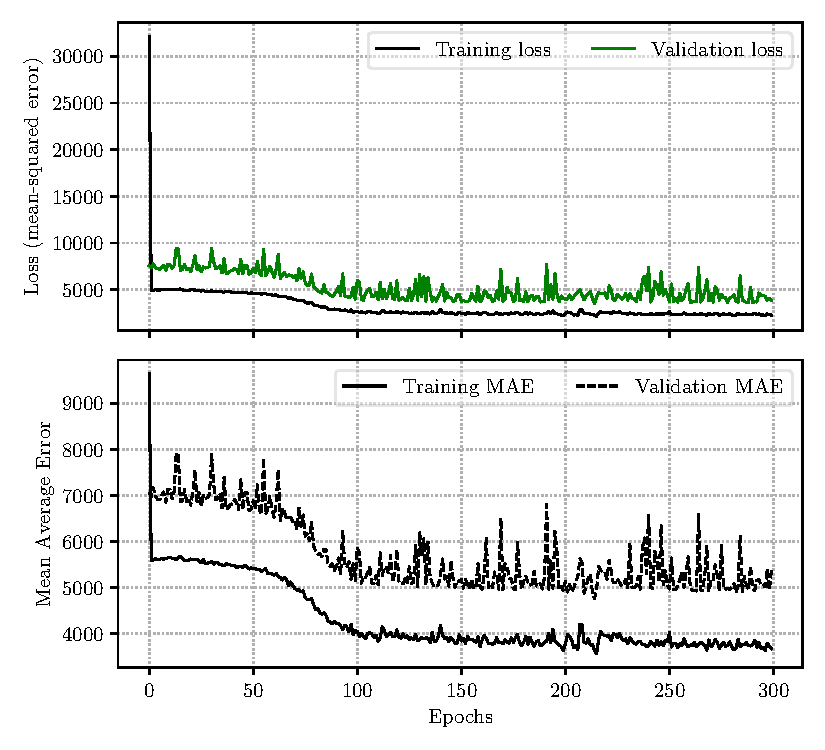
\includegraphics{figures/cmapss_regression_training.pdf}
    \caption{Training process of \acrshort{rul} predictor}
    \label{fig:cmapss-regression-training}
\end{figure}

After training, the model is evaluated on two units from the test set. Figure \ref{fig:cmapss-regression-prediction} shows the actual \acrshort{rul} (dashed line), model prediction at each cycle and a 3rd degree polyomial fit of model's predictions.

\begin{figure}[H]
    \centering
    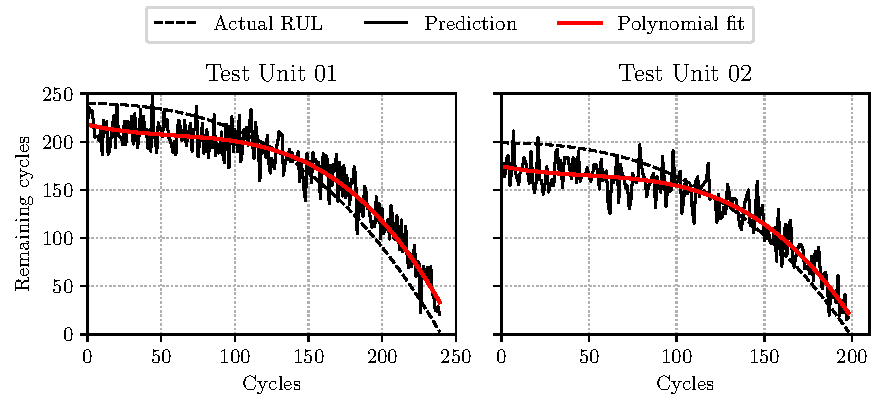
\includegraphics{figures/cmapss_regression_predictions.pdf}
    \caption{Prediction results on two test units}
    \label{fig:cmapss-regression-prediction}
\end{figure}

Although the model's prediction are close the the actual \acrshort{rul}, but they are noisy and there is so much fluctuation. The noise can be reduced by smoothing the output for example using moving average or fitting the points to a polynomial. But the reason of the noise in the first place is that fully-connected architecture doesn't take into consideration the previous predictions (i.e. acyclic architecture). Since \acrshort{rul} at each instant of time depends on the \acrshort{rul} from the previous one, taking previous steps into consideration while making new predictions can effectively reduce the noise and also improve prediction accuracy. To achieve that, a cyclic neural archtiecture like recurrent neural networks should be used.

\subsection{Improving \acrshort{rul} prediction using LSTM networks}
Fully-connected neural networks are powerful tool for modeling a wide range of problems, but using the fully-connected architecture for time series prediction, such as \acrshort{rul} prediction, can yield very noisy output because the network is acyclic and each instant in time is evaluated seperately and doesn't take into account the previous predictions. \acrlong{lstm} (Section \ref{section:lstm}) are a powerful tool for modeling such problems and to make more robust and less noisy predictions. In this section, fully-connected neural network architecture from previous section is replaced with an \acrshort{lstm} network to predict \acrshort{rul} in C-MAPSS dataset.

The architecure used here is described in Table \ref{table:cmapss-lstm-architecture}:

\begin{table}[h]
    \centering
    \begin{tabu}{lll}
		\tabucline[1.5pt]{-}
		\textbf{Layer (type)}   & \textbf{Output shape} &   \textbf{Param \#} \\
		\tabucline[1pt]{-}
		LSTM1 (LSTM) 			&   (None, 100, 100)    &       50000   \\
		LSTM2 (LSTM)           &   (None, 100, 100)    &       80400   \\
		LSTM3 (LSTM)           &   (None, 75)          &       52800   \\
        Dense1 (Dense)         &   (None, 120)         &       9120    \\
        Dense2 (Dense)         &   (None, 110)         &       13310   \\
        Dense3 (Dense)         &   (None, 100)         &       11100   \\
		\tabucline[1pt]{-}
		Total params: 216,730       &                   &               \\
		Trainable params: 216,730   &                   &               \\
		Non-trainable params: 0     &                   &               \\
	\tabucline[1.5pt]{-}
    \end{tabu}
    \caption{LSTM network architecture for \acrshort{rul} prediction}
    \label{table:cmapss-lstm-architecture}
\end{table}

It is apparent that the \acrshort{lstm} architecture has much more parameters (216,730 parameters) than fully-connected architecture (1,473). This is because of the more complicated design of \acrshort{lstm} cells and their possession of different gates. This results in much longer training time.

\acrshort{lstm} layers take 3 dimensional tensor as an input of shape \textit{(samples, sequence length, features)}. Sequence length was set to 100 in this architecture, that's why every training sample must have a shape of \textit{(sequence length, features)}. All units have the same number of features but different legnths, since every sample must have a sequence length of 100, samples with cycles less than 100 are padded with -10 where \acrshort{lstm} layers are set to ignore any time steps with this value.

The network was trained for 50 epochs with batch size of 16 and validation split of 0.2 using Adam optimizer. Training process is visualized in Figure \ref{fig:cmapss-lstm-training}:

\begin{figure}[H]
    \centering
    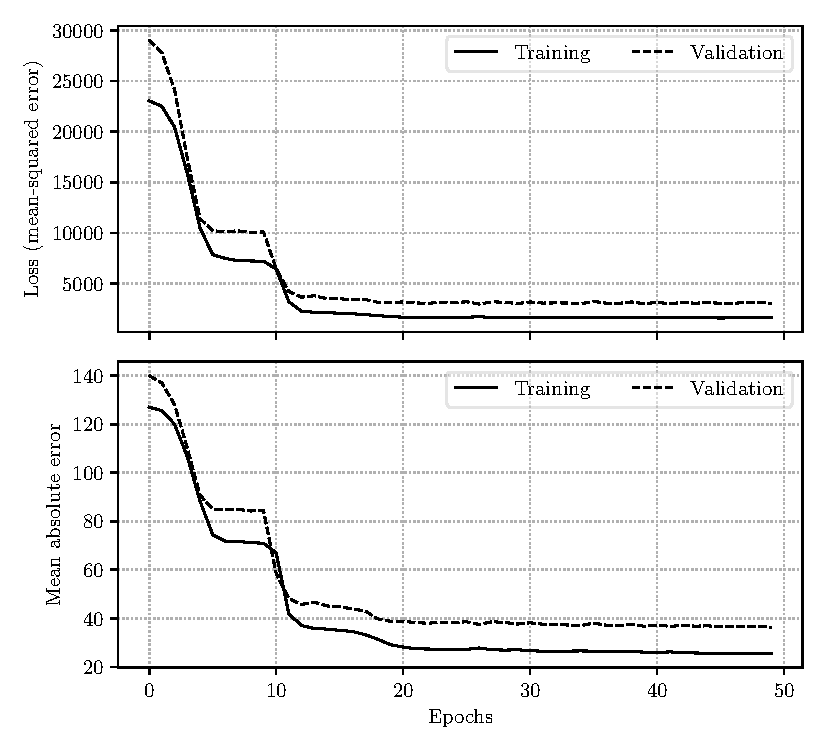
\includegraphics{figures/cmapss_lstm_training.pdf}
    \caption{LSTM training process}
    \label{fig:cmapss-lstm-training}
\end{figure}

Table \ref{table:cmapss-lstm-results} shows the loss and metric (i.e. mean absolute error) on the different train, validation and test sets:

\begin{table}[H]
	\centering
	\begin{tabu}{lcc}
		\tabucline[1.5pt]{2-3} 
						&	\textbf{Loss}	&	\textbf{Mean Absolute Error}	\\
	   \tabucline[1pt]{-}
		Train set 		&	1600.60			    &	25.43				\\
		Validation set 	&	3039.68 			&	36.37					\\
		Test set		&	1379.67 			&	23.27					\\
   \tabucline[1.5pt]{-}
   \end{tabu}
   \caption{\acrshort{lstm} training results}
   \label{table:cmapss-lstm-results}
\end{table}

Four different units were reserved as testing units, after training the network is used to predict \acrshort{rul} on test units. Figure \ref{fig:cmapss-lstm-prediction} shows prediction results and actual \acrshort{rul} of two different units.

\begin{figure}[h]
    \centering
    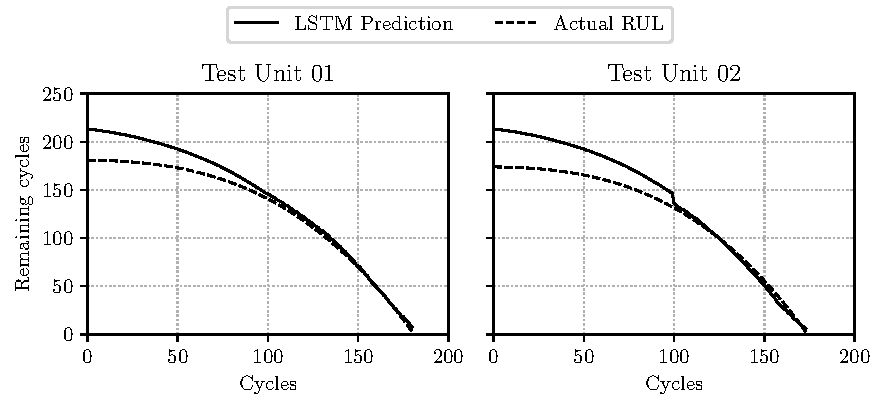
\includegraphics{figures/cmapss_lstm_regression_predictions.pdf}
    \caption{LSTM prediction results on two test units}
    \label{fig:cmapss-lstm-prediction}
\end{figure}

It's apparent that \acrshort{lstm} network predictions are much better and almost free of noise compared to those made by the fully-connected network shown in Figure \ref{fig:cmapss-regression-prediction}. Predicted \acrshort{rul} is almost identical to actual \acrshort{rul} towards the end of life of the unit.

\section{Conclusion}
Fully-connected neural networks are a powerful tool for quantifying health state of complex systems using condition monitoring data. C-MAPSS dataset is an example of a system with many interacting parts that provide a variety of condition-monitoring data (e.g. temperature, pressure, rpm, …) where the degradation isn't directly related to one component but is indicated by the sum of the trends in all the monitoring data. Neural networks are able to capture such trends and predict the \acrshort{rul} of the system before failure. Fully-connected networks were first used for this task, but a cyclic architecture like \acrshort{lstm} can produce better results with improved accuracy and much less noise.
\end{comment}
